% Argument and section organization adapted from Mucko (IJCAI 2020).
% All manuscript prose, tables, equations and bibliography reside here.
% Figure assets are stored in figures/; all sections remain in this main.tex.
% Compile twice with pdfLaTeX; cvpr.sty is the required conference style dependency.
\documentclass[10pt,twocolumn,letterpaper]{article}
\usepackage[review]{cvpr}
\usepackage{tabularx,array,newfloat,listings}
\usepackage{tikz}
\usetikzlibrary{arrows.meta,positioning,fit,calc}
\DeclareCaptionStyle{ruled}{labelfont=normalfont,labelsep=colon,strut=off}
\lstset{basicstyle=\footnotesize\ttfamily,showstringspaces=false,tabsize=4,breaklines=true,columns=fullflexible,keepspaces=true}
\DeclareFloatingEnvironment[name=Algorithm]{algorithm}
\captionsetup{hypcap=false}
\frenchspacing
\setcounter{secnumdepth}{2}
\definecolor{cvprblue}{rgb}{0.21,0.49,0.74}
\usepackage[pagebackref,breaklinks,colorlinks,allcolors=cvprblue]{hyperref}
\def\paperID{*****}
\def\confName{CVPR}
\def\confYear{2026}
\title{LegalFactAware: Summary-Level Membership Supervision for Fixed-Budget Extractive Summarization}
\author{Anonymous Authors}
\begin{document}
\maketitle


\begin{abstract}
Fixed-budget extractive summarization requires choosing complementary content that fits within a short output. Independent sentence--reference labels can favor overlapping candidates, while truncating a selected summary can remove part of its content. We introduce LegalFactAware, which combines summary-level membership supervision with complete-sentence budget decoding in a static scoring pipeline. A reference-guided greedy Oracle selects a sentence set whose members supply binary training targets. A linear scorer uses position-augmented lexical features and supplementary domain and passage-role cues; redundancy-aware fit/skip decoding then assembles complete candidates in source order. On CAIL2020-SFZY-clean under a 450-character, eight-sentence protocol, the method obtains ROUGE-1/2/L of 60.94/42.10/50.73 and rule-based Fact Recall of 70.99. Development controls favor the complete labeling procedure over independent weak supervision by 6.24/8.28/8.68 ROUGE points. Fit/skip raises Fact Recall by 4.06 points over tail truncation and reduces truncated outputs from 379 of 942 to zero. Matched controls find no statistically supported independent gain from the Oracle character budget or exact static-score knapsack selection. The findings support summary-level target construction combined with feasible complete-sentence decoding in the evaluated Chinese task.
\end{abstract}

\section{Introduction}\label{introduction}
Extractive summarization forms a concise account of a document by selecting its source sentences. A fixed output budget makes the contribution of a sentence depend on the other selected content: relevance alone does not determine which combination uses the available space well. The task also requires a selection procedure that can retain its chosen units in full. Training targets and output construction therefore provide two connected opportunities to improve a sentence-scoring pipeline.

Consider the schematic example in Figure~\ref{fig:motivation}. Candidates $s_1$ and $s_2$ both express road-closure content A, while $s_3$ adds service-resumption content B. With the character counts shown, choosing $s_1+s_2$ uses the same budget as choosing $s_1+s_3$, yet only the latter retains both content types. The example separates individual relevance from contribution to a summary combination. A useful training target should reflect how reference content has already been covered when another sentence is considered.

\begin{figure}[t]
\centering
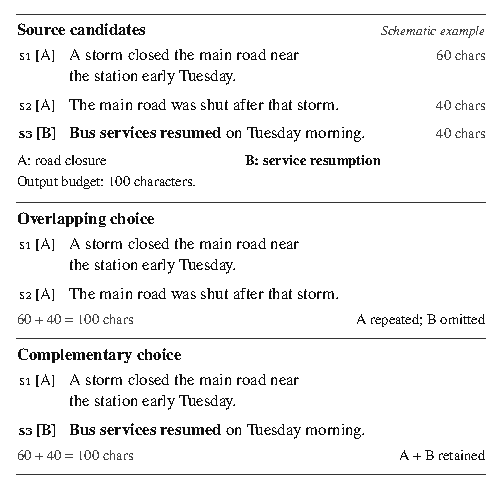
\includegraphics[width=\columnwidth]{figures/motivation.pdf}
\caption{Schematic content competition under a fixed budget. Underlined phrases express road closure (A); bold phrases express service resumption (B). Both complete-candidate combinations use 100 characters, counting spaces and punctuation without added separators.}\label{fig:motivation}
\end{figure}

Existing extractors address selection through contextual representations, extraction history and task-specific guidance. BERTSUM uses document context to estimate sentence salience \citep{ref1}; MemSum and SummaRuNNer incorporate previously extracted or accumulated content \citep{ref2,summarunner2017}. Strict-length extraction and budget-guided construction treat output space explicitly \citep{ref8,ref9}, and SENDE uses reference-guided Oracle labels for legal extraction \citep{ref5}. These approaches provide distinct mechanisms for improving sentence selection. Within a fixed static-scoring architecture, the remaining question is how reference summaries should define the training target and how scored candidates should be assembled under the output limits.

Independent weak labels compare each sentence with a reference separately, so overlapping candidates can all become positive without competing for a summary. A summary-level Oracle instead evaluates the gain from adding a candidate to the content already selected. Output construction poses a second issue: choosing sentences first and cutting the concatenated text afterward can remove the end of a selected candidate. Checking complete-candidate feasibility during selection allows another candidate to compete when one is too long. These mechanisms motivate separate tests of the labeling procedure and the decoder.

We propose LegalFactAware to study this combination. First, an offline reference-guided Oracle constructs a selected set and converts its members into sentence-wise targets. Second, a linear scorer uses position-augmented lexical features with supplementary domain and passage-role cues, and a redundancy-aware fit/skip decoder constructs the output. The scorer predicts individual membership probabilities; the decoder updates redundancy and remaining space after each choice. We evaluate the approach on Chinese legal judgments, using controlled substitutions and matched comparisons to distinguish the complete pipeline effects from the contribution of the Oracle character budget alone.

Our contributions are threefold. (1) We formulate summary-level membership supervision for a static sentence scorer and compare the complete label-construction procedure with independent weak supervision. (2) We combine this target construction with redundancy-aware complete-sentence selection that enforces the character and sentence limits during decoding. (3) We provide component, matched-control and case analyses that identify the main lexical representation benefit and establish the scope of the design effects: the Oracle budget toggle and exact additive-score optimization yield no statistically supported independent gain.

\section{Related Work}\label{related-work}
\textbf{Sentence representation and selection.} Contextual encoders improve the information available to a sentence scorer. BERTSUM combines pretrained representations with inter-sentence Transformer layers \citep{ref1}. Sequential extractors model the evolving summary: MemSum uses local content, document context and extraction history \citep{ref2}, while SummaRuNNer incorporates accumulated-summary information \citep{summarunner2017}. Legal summarizers also supply structural, rhetorical-role or terminology guidance \citep{ref6,ref3,ref4}; SSE models explicit summary structure \citep{ref7}. LegalFactAware uses lexical, domain and coarse role features in a static scorer. Its selected set changes decoding utility and feasibility, while the classifier scores themselves remain fixed.

\textbf{Reference-guided supervision.} Reference summaries can supply extraction targets even when sentence labels are unavailable. Independent sentence-level rules measure each candidate separately; Oracle procedures derive targets from a selected combination. SENDE already uses Oracle supervision \citep{ref5}. Its published Algorithm~1 matches the longest remaining reference unit to source candidates and recursively processes the remaining slices. Our procedure selects by marginal ROUGE of the accumulated summary with explicit character and sentence limits. The distinction is the label-construction program, rather than the use of an Oracle itself; a matched budget toggle further tests the character constraint within our program.

\textbf{Budgeted summary construction.} Supervised extraction under strict length limits \citep{ref8} and FactorSum's content and budget guidance \citep{ref9} establish output space as part of summary construction. Maximal marginal relevance (MMR) balances relevance and selected-content redundancy \citep{mmr1998}; LegalFactAware uses this trade-off with whole-candidate fit checks. Tail truncation, feasible greedy selection and exact additive-score selection answer different output-construction questions. We compare them under specified controls to separate candidate completeness from the choice of feasible selector, while retaining a static scoring architecture.

\section{Methodology}\label{legalfactaware}
Given ordered candidates $D=(s_1,\ldots,s_n)$, the task selects an index set $I\subseteq\{1,\ldots,n\}$. The summary $S(I)$ concatenates stored candidates in source order without added separators. For length function $L$, character budget $B$ and sentence cap $K$, the feasible sets are
\begin{equation}
\mathcal{F}(B,K)=\{I:L(S(I))\leq B,\ |I|\leq K\}.
\end{equation}
The Chinese experiments use Python string length, including stored whitespace, so $L(S(I))=\sum_{i\in I}|s_i|$, with $B=450$ and $K=8$. Figure~\ref{fig:method} shows summary-level target construction in panel (a), candidate representation and scorer learning in panel (b), and output selection in panel (c). Training uses references to construct membership targets; inference uses the fitted representation and scorer to choose a feasible output without a reference.

\begin{figure*}[t]
\centering
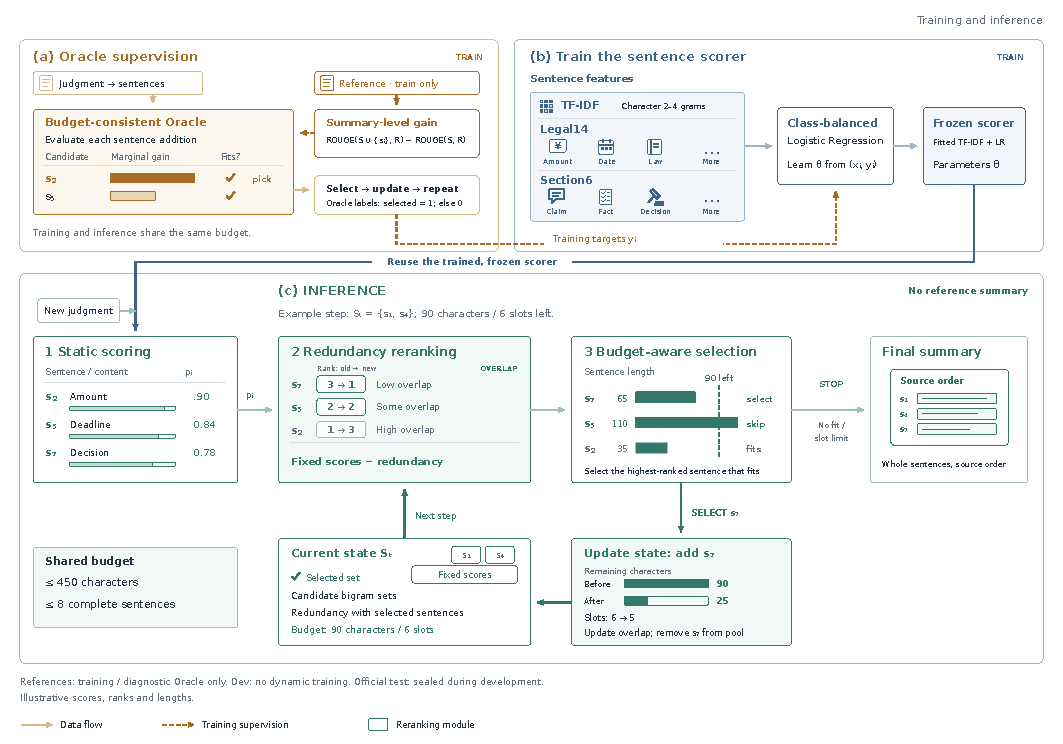
\includegraphics[width=\textwidth]{figures/method.pdf}
\caption{LegalFactAware training and inference. (a) A reference-guided greedy Oracle constructs binary membership targets. (b) Sentence features train a static scorer. (c) Fixed sentence scores are adjusted for overlap with selected sentences, followed by complete-sentence fit/skip. Selection updates the overlap state and remaining budget. Displayed scores, ranks and lengths are schematic.}\label{fig:method}
\end{figure*}

\subsection{Candidate Representation}\label{candidate-representation-and-scoring}
Candidate features retain detailed wording and source location, supplemented by compact domain and passage-role cues. This combination provides a fixed input to the scorer while allowing feature removal to test the contribution of each block.

\textbf{Position-augmented lexical features.} We prepend the zero-based marker \texttt{position\{index\}} and one space to each stored candidate, then apply character 2--4-gram term frequency--inverse document frequency (TF--IDF). We call this block position-augmented TF--IDF because the same vector represents both candidate wording and its prepended position marker. The vectorizer is fitted on training candidates and frozen for development and test; Appendix~G records its configuration.

\textbf{Legal and positional cues (Legal14).} The name Legal14 denotes a fourteen-dimensional feature vector: two relative-position values, log sentence length, five expression indicators, five capped expression counts, and expression-type diversity. The five expression types are money, dates, legal instruments, statutory articles and judicial-action terms. These cues supplement lexical detail with location and domain expressions; the latter give FactAware its operational meaning as scorer inputs. Appendix~B defines all fourteen dimensions.

\textbf{Passage-role cues (Section6).} Section6 is the shorthand for six-dimensional passage-role cues: Claim, Defense, Fact, Reason, Decision and Other. The number 6 denotes these six categories. A deterministic left-to-right marker scan assigns one role to each candidate. The state starts at Other and persists until a new marker appears; precedence is Decision, Reason, Fact, Defense, Claim. Standalone action terms trigger Decision only in the final 35\% of the document. The assigned role is encoded as a one-hot vector with one active entry among the six categories. This vector supplements lexical features with coarse passage function and is concatenated with the other blocks:
\begin{equation}
\mathbf{x}_i=[\mathbf{v}^{\mathrm{tfidf}}_i;\mathbf{f}^{\mathrm{legal}}_i;\mathbf{f}^{\mathrm{section}}_i].
\end{equation}
Here $\mathbf f_i^{\mathrm{legal}}\in\mathbb R^{14}$ denotes Legal14 and $\mathbf f_i^{\mathrm{section}}\in\{0,1\}^6$ denotes the Section6 passage-role vector. Thus the scorer receives one candidate vector combining lexical detail with coarse cues. Roles affect scoring through this vector; the decoder applies no role quotas.

\subsection{Summary-Level Membership Supervision}\label{budget-consistent-oracle-supervision}
Summary-level membership supervision labels each candidate by whether it belongs to a reference-guided sentence combination. The greedy target constructor is called an Oracle because it uses the reference summary to construct training targets offline. It measures the additional reference content captured after the current selection.

\textbf{Summary-level objective.} For reference $R$, the Oracle uses character-level ROUGE-1 and ROUGE-2 F1:
\begin{equation}
Q(S(I),R)=R1_{F1}(S(I),R)+R2_{F1}(S(I),R).
\end{equation}
The marginal gain of candidate $i$ after set $I_t$ is
\begin{equation}
\Delta(i\mid I_t)=Q(S(I_t\cup\{i\}),R)-Q(S(I_t),R).
\end{equation}
Previously covered content affects this gain, making overlapping candidates compete during target construction.

\textbf{Feasible greedy construction.} Starting from $I_0=\varnothing$, the Oracle adds the candidate with the largest strictly positive gain among additions in $\mathcal F(B,K)$. Candidates are scanned in source order, which resolves exact ties in favor of the earlier sentence. Selection stops at $K$, when no complete candidate fits, or when no feasible addition improves $Q$. Appendix~A specifies the deterministic procedure.

\textbf{Membership targets.} The final set defines
\begin{equation}
y_i=\mathbf1[i\in I_{\mathrm{orc}}].
\end{equation}
A selected sentence receives $y_i=1$ and every other candidate receives $y_i=0$. These sentence-wise targets carry the result of summary-level selection into scorer training. The classifier learns individual membership probabilities; the Oracle trajectory constructs labels offline. References are used for target construction and evaluation.

\subsection{Complete-Sentence Budget Decoding}\label{redundancy-and-complete-sentence-fitskip-decoding}
The static sentence scorer assigns each candidate a probability $p_i$ that remains fixed throughout decoding. The decoder assembles complete candidates while accounting for selected-content redundancy. It combines fixed classifier scores with a utility that changes after each accepted candidate, so high-scoring overlap and remaining space can affect later choices.

\textbf{Redundancy-adjusted utility.} Utility is the selection-time ranking score combining classifier probability and selected-content overlap. Within each document, normalize $p_i$ as $\widetilde p_i=(p_i-p_{\min})/(p_{\max}-p_{\min})$, using $0.5$ when all scores are equal. Let $G_i$ be the set of character bigrams after whitespace removal, and $J(i,j)=|G_i\cap G_j|/|G_i\cup G_j|$, with zero for an empty union. The MMR-style utility \citep{mmr1998} is
\begin{equation}
U(i\mid I_t)=\widetilde p_i-\lambda\max_{j\in I_t}J(i,j),
\end{equation}
where redundancy is zero for the empty selected set and $\lambda=0.2$. Using the maximum overlap penalizes a near duplicate even when other selected candidates discuss different content.

\textbf{Complete-sentence fit/skip selection.} Here \emph{fit} means accepting a complete candidate within the remaining character and sentence limits; \emph{skip} means passing over an overlong candidate so another can compete. At each round, choose the highest-utility unselected candidate whose inclusion remains in $\mathcal F(B,K)$; source order breaks ties. Utility is a ranking score and need not be positive. The decoder stops at the sentence cap or when no remaining complete candidate fits. Legal14 affects $p_i$ through the classifier, with no added fact-coverage reward at decoding.

\textbf{State and output.} An accepted candidate updates $I_t$, redundancy and remaining space while $p_i$ stays fixed. Selected candidates are returned verbatim in source order, preserving the units supplied by corpus segmentation, including headings or clauses. Feasibility therefore holds by construction. Direct decoding uses at most $O(K^2n)$ selected-candidate overlap computations; Oracle construction uses at most $O(Kn)$ summary evaluations, excluding length-dependent operation costs.

\subsection{Learning}\label{learning}
We fit one logistic-regression scorer to the candidate features and Oracle labels. Its static probabilities provide the common starting point for the decoder controls:
\begin{equation}
p_i=\sigma(\mathbf w^\top\mathbf x_i+b).
\end{equation}
For $M$ training candidates, class counts $M_0,M_1$, and balanced weights $a_c=M/(2M_c)$, the data loss is
\begin{equation}
\mathcal L_{\rm data}=-\sum_{i=1}^M[a_1y_i\log p_i+a_0(1-y_i)\log(1-p_i)].
\end{equation}
The L2-regularized model uses liblinear, $C=1.0$, an intercept, tolerance $10^{-4}$, at most 1,000 iterations and seed 42. Continuous scores are retained for ranking. The fitted scorer and training-fitted vectorizer are frozen during evaluation, allowing controls to replace targets, features or selection procedures within the same scoring architecture.

\section{Experiments}\label{experiments}
\textbf{Dataset.} We use CAIL2020-SFZY-clean, the supplied cleaned partition of the official Chinese judicial summarization resources \citep{ref12}: 7,495 training, 942 development and 948 test judgments. The test set has 53,318 candidates, averaging 56.24 per document. The corpus audit reports no empty documents or cross-split overlap in IDs, exact texts or near duplicates. Overall comparisons use the frozen test set; component, matched-control, case and budget analyses use development data. Appendix~C gives corpus statistics.

\textbf{Evaluation metrics.} We report document-macro ROUGE-1/2/L F1 \citep{rouge2004}, rule-based Fact Recall and Fact F1, plus budget violations and partial-candidate truncations. ROUGE uses Lawa 1.2.6; the Oracle uses a separate character-level objective. Expression metrics use the matching and averaging rules in Appendix~G. Practitioner-oriented evaluation and factual-consistency research distinguish automatic overlap from expert assessment \citep{ref10,ref11}; our expression scores measure detected reference content and source support.

\textbf{Implementation details.} The output cap is 450 stored-string characters and eight candidates. Internal controls retain the split and linear scoring architecture. Primary development tests use 10,000 paired bootstrap resamples and two-sided Wilcoxon tests with Pratt zeros; Holm correction covers 15 ROUGE contrasts. The two matched controls each report a separate four-metric correction family. Original and reconstructed artifacts, inference settings and statistical records are specified in Appendices~F--H.

\subsection{Comparison with Evaluated Methods}\label{overall-comparison-competitive-performance-within-the-target-budget}
Table~\ref{tab:1} compares supervised task adaptations \citep{ref3,ref4,ref13}, retrained official MemSum \citep{ref2}, the independent SENDE reconstruction \citep{ref5}, an SSE structural proxy \citep{ref7}, and LexRank adapted from the EUR-Lex-Sum setup \citep{lexrank2004,ref14}. CivilSum LED-tail and Budget Recipe are listed as generative references \citep{ref15,ref16}. LegalFactAware obtains 60.94/42.10/50.73 ROUGE and 70.99 Fact Recall, with zero budget violations and truncations. Its ROUGE gaps over the SSE proxy are 3.80/4.85/4.48 points, and over retrained MemSum 11.38/13.94/12.21. Agarwal-ST has similar expression recall (70.69), while LegalFactAware has higher ROUGE by 5.96/6.20/5.07 points.

SENDE is the closest ROUGE comparator at 59.72/41.13/50.65, leaving gaps of 1.22/0.97/0.08 points. The small ROUGE-L difference indicates competitive means; paired significance for SENDE is not reported. Systems share splits and nominal output caps, with different adaptation histories and preprocessing: SENDE strips whitespace, while LegalFactAware counts stored strings. Its Fact Recall of 66.91 is recomputed with the shared expression evaluator. Appendix~C identifies each implementation and the separate reconstructed paired comparisons. These results establish the evaluated pipeline's overall performance; the following controls examine which changes contribute to it.
\begin{table*}[!t]
\caption{Frozen CAIL2020-SFZY-clean test results (\%). Extractive implementations and generative references are grouped separately. Experimental status identifies each evaluated adaptation or reconstruction.}\label{tab:1}
\begin{tabularx}{\textwidth}{@{}>{\raggedright\arraybackslash}p{.25\textwidth}>{\raggedright\arraybackslash}Xrrrr@{}}
\toprule
\textbf{Method} & \textbf{Experimental status} & \textbf{R1} & \textbf{R2} & \textbf{RL} & \textbf{Fact Recall} \\
\midrule
\textbf{LegalFactAware v2.5-B} & \textbf{Proposed method} & \textbf{60.94} & \textbf{42.10} & \textbf{50.73} & \textbf{70.99} \\
SENDE & Independent task reconstruction & 59.72 & 41.13 & 50.65 & 66.91 \\
SSE & Structural proxy adaptation & 57.14 & 37.25 & 46.25 & 61.47 \\
Agarwal-ST & Constrained ST+MMR & 54.98 & 35.90 & 45.66 & 70.69 \\
TermDiffuSum & Independent reimplementation & 54.55 & 34.98 & 43.80 & 60.21 \\
Gist & Language/budget adaptation & 53.62 & 34.35 & 44.27 & 69.42 \\
MemSum & Official architecture retrained & 49.56 & 28.16 & 38.52 & 55.66 \\
EUR-Lex-Sum LexRank & Graph-ranking adaptation & 42.18 & 21.23 & 29.84 & 36.91 \\
\midrule
\multicolumn{6}{@{}l}{\textit{Generative reference systems}} \\
CivilSum LED-tail & Generative reference track & 53.57 & 28.59 & 41.35 & 43.60 \\
Budget Recipe & Zero-shot generative transfer & 40.19 & 19.05 & 26.26 & 33.46 \\
\bottomrule
\end{tabularx}
\end{table*}

\begin{table*}[!t]
\caption{Development controls (\%, 942 documents). Each row changes the named aspect relative to the full system. The feature blocks are position-augmented TF--IDF, fourteen-dimensional legal and positional cues (Legal14), and six-dimensional passage-role cues (Section6); supervision and tail truncation are procedure replacements. Fact F1 macro-averages type-level F1 scores (Appendix~G). Truncated counts partial-sentence outputs.}\label{tab:2}
\begin{tabular*}{\textwidth}{@{\extracolsep{\fill}}>{\raggedright\arraybackslash}p{.34\textwidth}rrrrrr@{}}
\toprule
\textbf{Variant} & \textbf{R1} & \textbf{R2} & \textbf{RL} & \textbf{Fact Recall} & \textbf{Fact F1} & \textbf{Truncated} \\
\midrule
\textbf{Full LegalFactAware} & \textbf{60.27} & \textbf{41.17} & \textbf{49.84} & \textbf{70.21} & \textbf{47.85} & \textbf{0} \\
\midrule
\multicolumn{7}{@{}l}{\textit{Supervision replacement}} \\
Independent sentence-level weak supervision & 54.03 & 32.89 & 41.17 & 59.90 & 39.85 & 0 \\
\midrule
\multicolumn{7}{@{}l}{\textit{Feature-block removal}} \\
Without position-augmented TF--IDF & 51.06 & 30.61 & 39.11 & 59.78 & 40.61 & 0 \\
Without legal/positional cues (Legal14) & 60.21 & 41.09 & 49.81 & 69.88 & 47.74 & 0 \\
Without passage-role cues (Section6) & 60.00 & 40.73 & 49.41 & 69.71 & 47.69 & 0 \\
Without Legal14 and Section6 cues & 59.90 & 40.66 & 49.27 & 69.04 & 47.33 & 0 \\
\midrule
\multicolumn{7}{@{}l}{\textit{Decoder replacement}} \\
Post-hoc tail truncation & 59.39 & 40.44 & 48.66 & 66.15 & 45.50 & 379 \\
\bottomrule
\end{tabular*}
\end{table*}


\subsection{Ablation Study}\label{controlled-changes-what-explains-the-gains}
We test supervision, representation and decoding separately in Table~\ref{tab:2}, then use matched controls to isolate the Oracle character budget and the feasible-selector choice.

\textbf{Supervision.} Replacing summary-level membership labels with independent weak labels lowers ROUGE by 6.24/8.28/8.68 points and Fact Recall by 10.30 points. All three ROUGE contrasts meet the paired-interval and Holm-adjusted criterion. Marginal reference gain makes repeated content compete during Oracle construction, consistent with the value of the resulting targets. This contrast assesses the complete labeling procedure, including its different selection rule and positive-label density.

\textbf{Representation.} Removing position-augmented TF--IDF lowers ROUGE by 9.21/10.56/10.73 points, the largest feature-block effect. Its character n-grams retain detailed wording and position that the compact cues summarize more coarsely. Removing the passage-role cues (Section6) lowers ROUGE by 0.28/0.44/0.43 points, with ROUGE-2 and ROUGE-L supported after correction. The smaller effect is consistent with coarse roles supplementing lexical evidence. The legal/positional block (Legal14) and the ROUGE-1 passage-role contrast lack corrected statistical support. The feature results therefore favor a detailed lexical backbone with smaller role-related gains.

\textbf{Decoding.} Replacing full fit/skip with tail truncation lowers ROUGE by 0.88/0.74/1.19 points and Fact Recall by 4.06 points; all three ROUGE contrasts meet the criterion. Truncation affects 379 of 942 control outputs and none of the full outputs. Fit/skip changes which complete candidates can compete before output construction, explaining the procedural difference tested by this replacement.

\begin{table*}[!t]
\caption{Contrasting development cases. Reference content is condensed and output excerpts are translated; party identifiers are omitted. Lengths and expression metrics use original Chinese outputs. FR: Fact Recall; FF1: type-level Fact F1. These are selected qualitative illustrations.}\label{tab:cases}
\small
\begin{tabularx}{\textwidth}{@{}>{\raggedright\arraybackslash}p{.14\textwidth}>{\raggedright\arraybackslash}p{.23\textwidth}>{\raggedright\arraybackslash}X>{\raggedright\arraybackslash}X@{}}
\toprule
\textbf{Case} & \textbf{Reference / source outcome} & \textbf{Complete-candidate fit/skip} & \textbf{Tail truncation} \\
\midrule
Employment dispute &
The court finds no employment relationship with the defendant and dismisses the plaintiff's claims. &
\emph{In sum, no employment relationship or mixed employment existed \ldots\ The claims \ldots\ are not supported.} It also retains: \emph{The plaintiff's claims are dismissed.} &
The same concluding reasoning is retained, but the output ends: \emph{Under the Labor Contract Law, Article 7} [cut]. The dismissal order is absent. \\
\addlinespace
Diagnostics & Original output, 450-character limit &
450 characters, 6 candidates; no cut. FR 77.78; FF1 62.18. &
450 characters, 8 candidates; cut. FR 41.67; FF1 49.05. \\
\midrule
Loan dispute &
The source orders repayment and, if repayment fails, disposal of the mortgaged property with priority recovery up to CNY 1 million. The reference also summarizes these outcomes. &
The output ends: \emph{In summary, under the cited legal provisions, judgment is rendered as follows:} The operative repayment and collateral-disposal orders are absent. &
The output ends inside the legal-citation passage [cut]. It also omits the operative repayment and collateral-disposal orders. \\
\addlinespace
Diagnostics & Original output, 450-character limit &
444 characters, 8 candidates; no cut. FR 30.00; FF1 23.33. &
450 characters, 8 candidates; cut. FR 30.00; FF1 23.33. \\
\bottomrule
\end{tabularx}
\end{table*}

\textbf{Matched controls.} Removing only the character budget from the matched Oracle gives 60.34/41.27/49.99 ROUGE and 47.78 Fact F1, versus 60.27/41.17/49.84 and 47.85 with it. All four Holm-adjusted tests are nonsignificant. Labels agree for 99.62\% of candidates; 757 of 7,495 training documents (10.10\%) change their selection. In a separate selector comparison without redundancy reranking, greedy fit/skip obtains 60.12/41.06/49.75 ROUGE and 47.63 Fact F1. Exact 0/1 knapsack changes 221 of 942 outputs and raises their summed static scores, yet lowers the four metrics by 0.10/0.39/0.29/0.12 points; all corrected tests are nonsignificant. Both selectors have zero truncations and violations. Appendix~D gives full results, label audits and auxiliary controls.

The controls support the complete supervision and decoder replacements over their tested alternatives. They locate the main supervision finding in the label-construction procedure as a whole, and show that more exact optimization of an additive sentence score does not improve the measured summary quality here.

\subsection{Computational Cost Analysis}\label{computational-cost-analysis}
We measure two complementary costs on the frozen 942-document development set. Complete-pipeline time starts from the shared segmented JSONL files and includes method-specific preparation, training and prediction; it excludes data download, common corpus construction, software installation, pretrained-weight download and final ROUGE aggregation. Each method is run three times in a fresh process without reusing method-specific training artifacts. Unified-start inference loads and warms each trained system once, then repeats five times from the same segmented development input, rebuilding all development-dependent representations before scoring, complete-sentence decoding and prediction writing. Model loading is excluded from the inference column and reported in Appendix~\ref{appendix-j-computational-cost}. All measurements use the frozen configurations corresponding to the evaluated adaptations in Table~\ref{tab:1}.

\begin{table}[t]
\caption{Computational cost on 942 development documents (mean $\pm$ sample standard deviation; lower is better). The comparison covers five implementations with auditable end-to-end timing pipelines.}\label{tab:cost}
\footnotesize
\begin{tabular*}{\columnwidth}{@{\extracolsep{\fill}}lcc@{}}
\toprule
\textbf{Method} & \textbf{Pipeline (min) $\downarrow$} & \textbf{Inference (s) $\downarrow$} \\
\midrule
\textbf{SSE proxy} & \textbf{14.42 $\pm$ 0.06} & \textbf{4.00 $\pm$ 0.04} \\
\underline{LegalFactAware} & \underline{31.18 $\pm$ 0.09} & \underline{16.03 $\pm$ 0.06} \\
SENDE reconstruction & 34.19 $\pm$ 0.18 & 19.52 $\pm$ 0.38 \\
MemSum adaptation & 95.86 $\pm$ 0.46 & 35.78 $\pm$ 0.19 \\
TermDiffuSum reimpl. & 155.52 $\pm$ 0.05 & 1,341.11 $\pm$ 4.11 \\
\bottomrule
\end{tabular*}
\end{table}

Table~\ref{tab:cost} places LegalFactAware second in both measurements among the five audited implementations. Relative to the independent SENDE reconstruction, its complete-pipeline and batch-inference times are lower by 8.81\% and approximately 17.9\%, respectively; the SSE structural proxy has the lowest measured cost. These descriptive timings complement the quality results but do not establish globally optimal efficiency, single-request latency, energy efficiency or superiority to methods omitted because no comparable full implementation was available.

\subsection{Output Behavior Analysis}\label{output-behavior-analysis}
We examine how output constraints and candidate selection affect retained content. Test outputs average 394.13 characters and 7.78 candidates, using 87.58\% of the character budget. The eight-candidate cap is reached in 821 of 948 documents (86.60\%). Fit checks fail in 706 documents, with 29,969 failed checks including repeated candidates across rounds. These aggregates identify frequent cap and feasibility events; they do not establish whether relaxing the cap would admit more candidates. Source Fact Support is 100\% for detected output expressions, measuring surface provenance.


The paired development cases in Table~\ref{tab:cases} illustrate two outcomes. In the employment dispute, both decoders retain the concluding reasoning; fit/skip also retains the dismissal order, while truncation ends inside a statutory citation. Its six-candidate output differs from the eight-candidate control in both composition and cutoff. In the loan dispute, the full output preserves 444 characters across eight candidates but ends at the judgment introduction, omitting repayment and collateral-disposal orders. A trace skips the 126-character collateral order when 125 characters remain. Appendix~I gives IDs, case-selection criteria and validated candidate alignment. Complete-candidate feasibility preserves the chosen text, while dispositive coverage still depends on which candidates are chosen.

\subsection{Parameter Analysis}\label{budget-sensitivity-coverage-and-complete-sentence-feasibility}
We vary the development decoding budget from 200 to 450 while fixing the scorer trained at 450 and retaining the eight-candidate cap. ROUGE rises from 51.49/33.44/42.34 to 60.27/41.17/49.84 and Fact Recall from 52.01 to 70.21, with zero truncations and budget violations throughout. From 400 to 450, ROUGE-2, ROUGE-L and recall increase, whereas ROUGE-1 and Fact F1 decrease slightly from their 400-character peaks. More space improves detected-expression coverage without uniformly increasing F1. The archived $\lambda=0.0$--$0.4$ sensitivity changes each ROUGE metric by less than 0.2 points. Appendix~E reports the full budget curve. These analyses describe decoding sensitivity for the same scorer, rather than retraining at each output limit.

\section{Conclusion}\label{conclusion}
We presented LegalFactAware for fixed-budget extractive summarization, combining offline summary-level membership supervision with complete-sentence budget decoding. On the evaluated Chinese legal task, controlled substitutions favor the complete labeling procedure over independent weak supervision and fit/skip over tail truncation. Position-augmented lexical features provide the largest tested representation benefit. Matched controls find no statistically supported independent gain from the Oracle character budget, and exact additive-score knapsack selection does not improve on greedy feasible selection. In a five-implementation cost audit, LegalFactAware has the second-lowest complete-pipeline and batch-inference times, while the SSE proxy is faster. The study shows how summary-level targets can inform a static scorer and how feasible decoding can preserve selected candidates, while the failure case identifies remaining content-coverage limits. Extending this evidence to other languages and expert-assessed summary quality provides the next evaluation setting.

{\small
\begin{thebibliography}{20}
\providecommand{\natexlab}[1]{#1}
\providecommand{\url}[1]{\texttt{#1}}
\expandafter\ifx\csname urlstyle\endcsname\relax
  \providecommand{\doi}[1]{doi: #1}\else
  \providecommand{\doi}{doi: \begingroup \urlstyle{rm}\Url}\fi

\bibitem[Agarwal et~al.(2022)Agarwal, Xu, and Grabmair]{ref3}
A. Agarwal, S. Xu, and M. Grabmair.
\newblock {Extractive summarization of legal decisions using multi-task
  learning and maximal marginal relevance}.
\newblock In \emph{Findings of the Association for Computational Linguistics:
  EMNLP 2022}, pages 1857--1872, 2022.

\bibitem[Aumiller et~al.(2022)Aumiller, Chouhan, and Gertz]{ref14}
D. Aumiller, A. Chouhan, and M. Gertz.
\newblock {EUR-Lex-Sum: A multi- and cross-lingual dataset for long-form
  summarization in the legal domain}.
\newblock In \emph{Proceedings of the 2022 Conference on Empirical Methods in
  Natural Language Processing}, pages 7626--7639, 2022.

\bibitem[Carbonell and Goldstein(1998)]{mmr1998}
Jaime Carbonell and Jade Goldstein.
\newblock The use of {MMR}, diversity-based reranking for reordering documents and producing summaries.
\newblock In \emph{Proceedings of the 21st Annual International ACM SIGIR Conference on Research and Development in Information Retrieval}, pages 335--336, 1998.

\bibitem[Chaksangchaichot and Akarajaradwong(2025)]{ref16}
C. Chaksangchaichot and P. Akarajaradwong.
\newblock {A budget recipe for finetuning a long-form legal summarization
  model}.
\newblock In \emph{Proceedings of the 1st Workshop on NLP for Empowering
  Justice (JUST-NLP 2025)}, pages 113--120, 2025.

\bibitem[{{China AI and Law Challenge}}(2020)]{ref12}
{{China AI and Law Challenge}}.
\newblock {CAIL2020 official judicial summarization task resources}, 2020.\newblock \url{https://github.com/china-ai-law-challenge/CAIL2020/tree/master/sfzy}.

\bibitem[Dong et~al.(2025)Dong, Li, Le, Jiang, Zhong, and Wang]{ref4}
X. Dong, W. Li, Y. Le, Z. Jiang, J. Zhong, and Z. Wang.
\newblock {TermDiffuSum: A term-guided diffusion model for extractive
  summarization of legal documents}.
\newblock In \emph{Proceedings of the 31st International Conference on
  computational linguistics}, pages 3222--3235, 2025.

\bibitem[Erkan and Radev(2004)]{lexrank2004}
Gunes Erkan and Dragomir R. Radev.
\newblock {LexRank}: Graph-based lexical centrality as salience in text summarization.
\newblock \emph{Journal of Artificial Intelligence Research}, 22:457--479, 2004.

\bibitem[Fonseca et~al.(2022)Fonseca, Ziser, and Cohen]{ref9}
M. Fonseca, Y. Ziser, and S.~B. Cohen.
\newblock {Factorizing content and budget decisions in abstractive
  summarization of long documents}.
\newblock In \emph{Proceedings of the 2022 Conference on Empirical Methods in
  Natural Language Processing}, pages 6341--6364, 2022.

\bibitem[Gu et~al.(2022)Gu, Ash, and Hahnloser]{ref2}
N. Gu, E. Ash, and R. Hahnloser.
\newblock {MemSum: Extractive summarization of long documents using multi-step
  episodic Markov decision processes}.
\newblock In \emph{Proceedings of the 60th Annual Meeting of the association
  for computational linguistics (volume 1: Long Papers)}, pages 6507--6522,
  2022.

\bibitem[Lin(2004)]{rouge2004}
Chin-Yew Lin.
\newblock {ROUGE}: A package for automatic evaluation of summaries.
\newblock In \emph{Text Summarization Branches Out}, pages 74--81, 2004.

\bibitem[Liu and Chen(2019)]{ref13}
C.-L. Liu and K.-C. Chen.
\newblock {Extracting the gist of Chinese judgments of the supreme court}.
\newblock In \emph{Proceedings of the seventeenth International Conference on
  artificial intelligence and law}, pages 73--82, 2019.

\bibitem[Liu and Lapata(2019)]{ref1}
Y. Liu and M. Lapata.
\newblock {Text summarization with pretrained encoders}.
\newblock In \emph{Proceedings of the 2019 Conference on Empirical Methods in
  Natural Language Processing and the 9th International Joint Conference on
  Natural Language Processing (EMNLP-IJCNLP)}, pages 3730--3740, 2019.

\bibitem[Malik et~al.(2024)Malik, Zhao, Fonseca, Rao, and Cohen]{ref15}
M. Malik, Z. Zhao, M. Fonseca, S. Rao, and S.~B. Cohen.
\newblock {CivilSum: A dataset for abstractive summarization of Indian court
  decisions}.
\newblock In \emph{Proceedings of the 47th international ACM SIGIR conference
  on Research and Development in Information Retrieval}, pages 2241--2250,
  2024.

\bibitem[Mehdad et~al.(2016)Mehdad, Stent, Thadani, Radev, Billawala, and
  Buchner]{ref8}
Y. Mehdad, A. Stent, K. Thadani, D. Radev, Y. Billawala, and K. Buchner.
\newblock {Extractive summarization under strict length constraints}.
\newblock In \emph{Proceedings of the tenth International Conference on
  Language Resources and Evaluation (LREC’16)}, pages 3089--3093, 2016.

\bibitem[Mujahid et~al.(2026)Mujahid, Wright, and Augenstein]{ref11}
Z.~M. Mujahid, D. Wright, and I. Augenstein.
\newblock {Stress testing factual consistency metrics for long-document
  summarization}.
\newblock In \emph{Proceedings of the 64th Annual Meeting of the association
  for computational linguistics (volume 1: Long Papers)}, pages 31914--31933,
  2026.

\bibitem[Nallapati et~al.(2017)Nallapati, Zhai, and Zhou]{summarunner2017}
Ramesh Nallapati, Feifei Zhai, and Bowen Zhou.
\newblock {SummaRuNNer}: A recurrent neural network based sequence model for
  extractive summarization of documents.
\newblock In \emph{Proceedings of the AAAI Conference on Artificial
  Intelligence}, pages 3075--3081, 2017.

\bibitem[Shukla et~al.(2022)Shukla, Bhattacharya, Poddar, Mukherjee, Ghosh,
  Goyal, and Ghosh]{ref10}
A. Shukla, P. Bhattacharya, S. Poddar, R. Mukherjee, K. Ghosh, P. Goyal, and S.
  Ghosh.
\newblock {Legal case document summarization: Extractive and abstractive
  methods and their evaluation}.
\newblock In \emph{Proceedings of the 2nd Conference of the Asia-Pacific
  Chapter of the Association for Computational Linguistics and the 12th
  International Joint Conference on Natural Language Processing (volume 1: Long
  papers)}, pages 1048--1064, 2022.

\bibitem[Wang et~al.(2023)Wang, Wang, Zhao, Amor, Liu, Zheng, Zhang, and
  Huang]{ref7}
Q. Wang, R. Wang, K. Zhao, R. Amor, B. Liu, X. Zheng, Z. Zhang, and Z. Huang.
\newblock {Towards legal judgment summarization: A structure-enhanced
  approach}.
\newblock In \emph{ECAI 2023}, 2023.\newblock \doi{10.3233/FAIA230553}.

\bibitem[Xi et~al.(2026)Xi, Huang, Duan, and Zhang]{ref5}
T. Xi, R. Huang, Z. Duan, and J. Zhang.
\newblock {SENDE: Extractive summarization of legal documents by sentence
  noising-reconstruction and dilated-gated convolutional networks}.
\newblock \emph{The Journal of Supercomputing}, 82, Article 117, 2026.\newblock \doi{10.1007/s11227-026-08248-4}.

\bibitem[Zhong and Litman(2022)]{ref6}
Y. Zhong and D. Litman.
\newblock {Computing and exploiting document structure to improve unsupervised
  extractive summarization of legal case decisions}.
\newblock In \emph{Proceedings of the Natural Legal Language Processing
  Workshop 2022}, pages 322--337, 2022.

\end{thebibliography}
}

\appendix
\raggedbottom

\par\medskip\noindent\begin{minipage}{\columnwidth}
\section{Detailed Algorithms}\label{appendix-a-detailed-algorithms}

These procedures specify deterministic tie handling, Oracle stopping, and inference fit/skip decisions.


\hrule
\captionof{algorithm}{Budget-consistent Oracle}
\hrule
\begin{lstlisting}
Input: D, R, B, K (defined in Section 3)
Output: Oracle set I_orc and labels y

1  I <- empty; q <- Q(S(I), R)
2  while |I| < K:
3      best <- None; best_score <- q
4      for each i not in I, in source order:
5          I' <- sort(I union {i})
6          if L(S(I')) > B: continue
7          q' <- Q(S(I'), R)
8          if q' > best_score:
9              best <- i; best_score <- q'
10     if best is None: break
11     I <- I union {best}; q <- best_score
12 I_orc <- sort(I)
13 y_i <- 1 if i in I_orc, otherwise 0
14 return I_orc, y
\end{lstlisting}
\hrule


\end{minipage}\par\smallskip

\par\medskip\noindent\begin{minipage}{\columnwidth}
\hrule
\captionof{algorithm}{Redundancy-aware fit/skip decoding}
\hrule
\begin{lstlisting}
Input: D, p, B, K, lambda
       (defined in Section 3)
Output: extractive summary S

1  Normalize p within document to p_tilde
2  Build character-bigram sets G_i
3  I <- empty
4  while |I| < K:
5      best <- None; bestU <- -infinity
6      for unselected i, in source order:
7          I' <- sort(I union {i})
8          if L(S(I')) > B: continue
9          red <- 0
10         for j in I:
11             red <- max(red, Jaccard(G_i,G_j))
12         u <- p_tilde_i - lambda * red
13         if u > bestU:
14             best <- i; bestU <- u
15     if best is None: break
16     I <- I union {best}
17 return S(sort(I))
\end{lstlisting}
\hrule
\end{minipage}\par\smallskip

\par\medskip\noindent\begin{minipage}{\columnwidth}
\section{Legal and Positional Cue Definitions}\label{appendix-b-legal14-definitions}

Table~\ref{tab:4} defines the fourteen-dimensional legal and positional vector, abbreviated Legal14. Its dimensions comprise three position/length features, ten expression indicators and counts, and one expression-diversity feature. Counts are capped and scaled; indicators are binary.

\captionof{table}{Fourteen-dimensional legal and positional cues (Legal14).}\label{tab:4}
\begin{tabularx}{\columnwidth}{@{}l>{\raggedright\arraybackslash}X>{\raggedright\arraybackslash}X@{}}
\toprule
\textbf{No.} & \textbf{Feature} & \textbf{Definition} \\
\midrule
1 & Forward relative position & \(i/\max(n,1)\) \\
2 & Reverse relative position & \((n - i)/\max(n,1)\) \\
3 & Log sentence length & \(\log\left( 1 + \left| s_{i} \right| \right)/8\) \\
4 & Contains money & Binary indicator \\
5 & Money count & \(\min\left( c_{money},5 \right)/5\) \\
6 & Contains date & Binary indicator \\
7 & Date count & \(\min\left( c_{date},5 \right)/5\) \\
8 & Contains legal instrument & Binary indicator \\
9 & Legal-instrument count & \(\min\left( c_{law},5 \right)/5\) \\
10 & Contains statutory article & Binary indicator \\
11 & Statutory-article count & \(\min\left( c_{article},5 \right)/5\) \\
12 & Contains judicial-action term & Binary indicator \\
13 & Judicial-action count & \(\min\left( c_{action},5 \right)/5\) \\
14 & Fact-signal diversity & Number of non-empty signal types divided by 5 \\
\bottomrule
\end{tabularx}
\end{minipage}\par\smallskip

\par\medskip\noindent\begin{minipage}{\columnwidth}
\section{Dataset and Baseline Details}\label{appendix-c-dataset-and-baseline-details}

Tables~\ref{tab:5} and~\ref{tab:6} provide corpus statistics and executable-system identities. Table~\ref{tab:7} gives archived aligned means; Appendix~F records the reconstruction used for paired checks.

\captionof{table}{Statistics of CAIL2020-SFZY-clean.}\label{tab:5}
\begin{tabular}{@{}lrrr@{}}
\toprule
\textbf{Statistic} & \textbf{Train} & \textbf{Dev.} & \textbf{Test} \\
\midrule
Documents & 7,495 & 942 & 948 \\
Source sentences & 428,766 & 53,870 & 53,318 \\
Avg. sentences & 57.21 & 57.19 & 56.24 \\
Avg. source chars & 2,571.75 & 2,577.14 & 2,525.53 \\
Avg. reference chars & 283.19 & 283.49 & 283.63 \\
\bottomrule
\end{tabular}
\end{minipage}\par\smallskip

The reconstructed test predictions are aligned by document ID with preserved LegalFactAware-v2, CAIL-adapted MemSum and SSE-v2 outputs. All nine ROUGE contrasts have positive 95\% bootstrap intervals and Holm-adjusted Wilcoxon $p<0.05$. These checks concern the three named implementations; SSE-v2 differs from the structural SSE proxy in Table~\ref{tab:1}. Sentence F1 measures selection agreement against the evaluation sentence labels.

\par\medskip\noindent\begin{minipage}{\columnwidth}
\captionof{table}{Baselines and their experimental status. Extractive implementations are listed separately from generative references.}\label{tab:6}
\begin{tabularx}{\columnwidth}{@{}>{\raggedright\arraybackslash}p{0.29\columnwidth}>{\raggedright\arraybackslash}X@{}}
\toprule
\textbf{Method} & \textbf{Category and experimental status} \\
\midrule
LegalFactAware v2.5-B & Constrained-membership extraction. Proposed method. \\
SENDE & Supervised extraction. Constrained independent reconstruction. \\
SSE & Structure-inspired extractive proxy. Structural proxy adaptation. \\
Agarwal-ST & Sentence scoring + MMR. Constrained ST+MMR reimplementation. \\
TermDiffuSum & Term-diffusion extraction. Independent reimplementation. \\
Gist & Legal supervised extraction. Language and budget adaptation. \\
MemSum & Sequential extraction. Official architecture retrained. \\
EUR-Lex-Sum LexRank & Graph ranking. Language and budget adaptation. \\
CivilSum LED-tail & Long-text generation. Separate generative track. \\
Budget Recipe & LLM generation. Public-checkpoint zero-shot transfer. \\
\bottomrule
\end{tabularx}
\end{minipage}\par\smallskip

\par\medskip\noindent\begin{minipage}{\columnwidth}
\captionof{table}{Archived aligned test means (\%). Full: LegalFactAware v2.5-B; v2: LegalFactAware-v2; MemSum: CAIL adaptation; SSE-v2: independent reimplementation. FR: Fact Recall; SF1: Sentence F1.}\label{tab:7}
\begin{tabular*}{\columnwidth}{@{\extracolsep{\fill}}lrrrrr@{}}
\toprule
\textbf{Model} & \textbf{R1} & \textbf{R2} & \textbf{RL} & \textbf{FR} & \textbf{SF1} \\
\midrule
\textbf{Full} & \textbf{60.94} & \textbf{42.10} & \textbf{50.73} & \textbf{70.99} & \textbf{59.83} \\
v2 & 52.98 & 32.09 & 39.78 & 57.04 & 42.09 \\
MemSum & 49.56 & 28.16 & 38.52 & 55.66 & 41.15 \\
SSE-v2 & 49.89 & 28.73 & 36.95 & 55.13 & 41.13 \\
\bottomrule
\end{tabular*}
\end{minipage}\par\smallskip



\par\medskip\noindent\begin{minipage}{\columnwidth}
\section{Feature Interactions and Auxiliary Controls}\label{appendix-d-feature-interactions-and-auxiliary-controls}

Table~\ref{tab:8} reports the four combinations of legal/positional cues (Legal14) and passage-role cues (Section6) in the archived feature-control series.

\captionof{table}{Development feature combinations (\%). TF: position-augmented TF--IDF; L: fourteen-dimensional legal/positional cues (Legal14); S: six-dimensional passage-role cues (Section6); Full: TF+L+S. FR: Fact Recall; FF1: Fact F1.}\label{tab:8}
\begin{tabular*}{\columnwidth}{@{\extracolsep{\fill}}lrrrrr@{}}
\toprule
\textbf{Features} & \textbf{R1} & \textbf{R2} & \textbf{RL} & \textbf{FR} & \textbf{FF1} \\
\midrule
TF & 59.90 & 40.66 & 49.27 & 69.04 & 47.33 \\
TF+L & 60.00 & 40.73 & 49.41 & 69.71 & 47.69 \\
TF+S & 60.21 & 41.09 & 49.81 & 69.88 & 47.74 \\
\textbf{Full} & \textbf{60.27} & \textbf{41.17} & \textbf{49.84} & \textbf{70.21} & \textbf{47.85} \\
\bottomrule
\end{tabular*}
\end{minipage}\par\smallskip

Complete-sentence length-constrained selection without redundancy control obtains ROUGE-1/2/L of 60.12/41.06/49.75 with zero hard truncations. Adding redundancy control gives 60.27/41.17/49.84, also with zero hard truncations; mean inter-sentence repetition changes from 5.78\% to 5.37\%. This auxiliary contrast changes the redundancy term, while both variants enforce whole-sentence feasibility. Varying the coefficient from 0.0 to 0.4 changes each ROUGE metric by less than 0.2 points in the coefficient-sensitivity analysis. Without class balancing, ROUGE is 60.28/41.23/49.95 and Fact F1 is 47.56, compared with 47.85 for the balanced model. These observations do not establish an independent ROUGE gain from balancing.

\par\medskip\noindent\begin{minipage}{\columnwidth}
\captionof{table}{Matched development controls (\%, 942 documents). FF1: Fact F1. Oracle rows share the inference pipeline. Selector rows share static scores and omit redundancy reranking; their greedy baseline differs from the full system.}\label{tab:matched}
\small
\begin{tabular*}{\columnwidth}{@{\extracolsep{\fill}}lrrrr@{}}
\toprule
\textbf{Control} & \textbf{R1} & \textbf{R2} & \textbf{RL} & \textbf{FF1} \\
\midrule
\multicolumn{5}{l}{\emph{Training Oracle budget}} \\
450-character budget & 60.27 & 41.17 & 49.84 & 47.85 \\
No character budget & 60.34 & 41.27 & 49.99 & 47.78 \\
\midrule
\multicolumn{5}{l}{\emph{Static-score feasible selector}} \\
Greedy fit/skip & 60.12 & 41.06 & 49.75 & 47.63 \\
Exact 0/1 knapsack & 60.02 & 40.67 & 49.46 & 47.51 \\
\bottomrule
\end{tabular*}
\end{minipage}\par\smallskip

\textbf{Oracle budget toggle.} The matched summary-level procedure retains the reference objective, greedy selection, sentence cap, classifier and inference decoder while toggling the training character budget. Reconstructed budgeted labels exactly match the historical archive. Sentence-label agreement between budgeted and unbudgeted targets is 99.62\%, with positive-label Jaccard 96.66\%. The selected set changes in 757 of 7,495 training documents. Budgeted-minus-unbudgeted differences in ROUGE-1/2/L and Fact F1 are $-0.07/-0.10/-0.15/+0.07$ points; the corresponding Holm-adjusted $p$ values are 0.159/0.141/0.097/0.771. The four comparisons form the reported correction family.

\textbf{Exact additive-score selection.} Under the same static sentence scores, exact 0/1 knapsack changes 221 of 942 selected sets (23.46\%) relative to greedy fit/skip. It attains a higher summed sentence score in those documents, but its ROUGE-1/2/L and Fact F1 are lower by 0.10/0.39/0.29/0.12 points. Both methods yield zero budget violations and hard truncations. All four Wilcoxon--Holm comparisons are nonsignificant. The reported bootstrap analysis trends in favor of greedy selection for ROUGE-2 and ROUGE-L, while the corrected Wilcoxon criterion is not met; this result is not reported as a significant selector advantage. Both new controls use development data without accessing the test set.

\par\medskip\noindent\begin{minipage}{\columnwidth}
\section{Complete Budget Curve}\label{appendix-e-complete-budget-curve}

Table~\ref{tab:9} applies one frozen model to different development decoding limits; the model is not retrained at each budget.

\captionof{table}{Development budget sensitivity (\%). The upper panel reports ROUGE; the lower panel reports Fact Recall (FR), Fact F1 (FF1), and mean output characters.}\label{tab:9}
\begin{tabular*}{\columnwidth}{@{\extracolsep{\fill}}rrrr@{}}
\toprule
\textbf{Budget} & \textbf{R1} & \textbf{R2} & \textbf{RL} \\
\midrule
200 & 51.49 & 33.44 & 42.34 \\
250 & 55.89 & 36.47 & 45.52 \\
300 & 58.60 & 38.69 & 47.72 \\
350 & 59.94 & 40.10 & 49.05 \\
400 & \textbf{60.39} & 40.89 & 49.71 \\
450 & 60.27 & \textbf{41.17} & \textbf{49.84} \\
\midrule
\textbf{Budget} & \textbf{FR} & \textbf{FF1} & \textbf{Avg. chars} \\
\midrule
200 & 52.01 & 44.31 & 197.23 \\
250 & 57.96 & 46.35 & 246.34 \\
300 & 62.41 & 47.40 & 293.56 \\
350 & 66.13 & 47.93 & 336.18 \\
400 & 68.71 & \textbf{47.98} & 370.49 \\
450 & \textbf{70.21} & 47.85 & 396.49 \\
\bottomrule
\end{tabular*}
\end{minipage}\par\smallskip

At 450 characters, average development output length is 396.49, leaving 53.51 characters unused. The test evaluator detects 32.41 unique source fact items per document on average. Fact Recall uses detected reference items as its denominator; the source-item count describes the input documents.

\section{Reproducibility and Artifact Provenance}\label{appendix-f-reproducibility-and-batch-record}
\textbf{Frozen inputs and environment.} Development controls use batch \texttt{LegalFactAware-\allowbreak v2.5-B-\allowbreak formal-dev-\allowbreak ablation-\allowbreak 20260821}, with 7,495 training documents, 942 development documents and 428,766 training candidates. The archived development configuration records Python 3.10.8 and scikit-learn 1.7.2. The separately documented reconstruction uses Python 3.10.19, scikit-learn 1.7.2, SciPy 1.15.3, NumPy 2.2.6 and Lawa 1.2.6. Split, model and record digests below identify the audited inputs and outputs.

\textbf{Independent-label control.} After whitespace removal, clipped character-bigram overlap is divided by the number of candidate bigrams. A sentence receives a positive label exactly when this precision exceeds 0.1. The rule yields 66.54\% positive training candidates and 38.06 positives per document, compared with 11.00\% and 6.29 for constrained Oracle membership.

\textbf{Statistical protocol.} The archived recomputation used 942 ID-aligned development records, 10,000 paired bootstrap resamples, seed 42 and two-sided paired Wilcoxon tests with Pratt zero handling. Holm correction covers 15 primary development ROUGE tests (five variants $\times$ three metrics). Test checks cover nine comparisons against three preserved baselines. Appendix~G defines the interpretation criterion, and Appendix~H gives the development effects and intervals.

\textbf{Reconstruction and archived results.} The historical final-model binary and original prediction bundle are unavailable. A separately recorded reconstruction uses unchanged v2.5 features and decoding, the verified v2.2 vectorizer and the rebuilt v2.5-B classifier. Its 948 unique ID-aligned test predictions obtain ROUGE-1/2/L of 60.9391/42.0963/50.7268 and Fact Recall of 70.9913. Maximum archived ROUGE deviation is 0.00056 percentage points; Sentence F1 is 59.82 versus the archived 59.83. Paired significance checks concern LegalFactAware-v2, MemSum and SSE-v2; the SSE proxy in Table~\ref{tab:1} is a different implementation. The SENDE comparison reports test means without a paired significance result.

\textbf{Verified development outputs.} The supplied verification bundle contains 942 unique records for each of the full predictions, tail-truncation predictions and archived full-model LAWA metrics. IDs, sources, references, model identifiers and budgets agree across paired predictions. Its eight file digests match the supplied checksum list; the three JSONL digests also match the archived manifest. Recomputing expression metrics gives full-system Fact Recall/Fact F1 of 70.2051/47.8526 and tail-truncation values of 66.1500/45.5041, with 0/379 hard truncations. Archived document-level ROUGE averages reproduce the displayed full-model means. All 29,324 logged development fit failures have candidate length above remaining space and utility equal to normalized score minus $0.2$ times redundancy. The fact reward is zero.

\textbf{SENDE reconstruction and verification.} The supplied code and records identify run \path{sende_independent_20260826}. Preparation removes all whitespace from source sentences and references. Its recursive Oracle filters candidates by positive reference ROUGE-2, matches the longest reference unit using $0.4R_1+0.3R_2+0.3R_L$, and recurses over nonoverlapping source/reference slices. This label procedure has no character budget or sentence cap. Chinese legal RoBERTa receives one epoch of TSDAE adaptation over 428,766 training sentences (maximum 128 tokens, batch 64, learning rate $2\times10^{-5}$). The six-layer gated CNN uses 768-dimensional embeddings, hidden size 384, dilations $[1,2,4,8,1,1]$, dropout 0.1, weighted binary cross-entropy and AdamW at $2\times10^{-4}$ (batch 64). Seed 20260826 partitions the 7,495 training documents into 7,120 fitting and 375 validation documents. Early stopping selects epoch three from six executed epochs. The separate 942-document development set selects probability threshold 0.8 from $\{0.1,\ldots,0.9\}$ by mean ROUGE. Inference ranks eligible sentences by probability, applies complete-sentence fit/skip at 450 characters and eight sentences, and restores source order. Thus SENDE also enforces feasible complete-sentence output; the comparison evaluates different labeling and scoring pipelines.

The 948 test predictions exactly reconstruct from their recorded source indices and satisfy both output caps. Their archived per-document ROUGE averages agree with the evaluation log and \path{results.json}: 59.72/41.13/50.65. Applying the shared expression functions to stored predictions and references gives Fact Recall 66.90699 and Fact F1 45.12947. Table~\ref{tab:1} adds the rounded Fact Recall; ROUGE is aggregated from archived scores rather than rerun through Lawa. The bundle supplies the CNN checkpoint, preparation/training/evaluation code and manifests; the adapted encoder weights and embedding arrays are absent, so this audit verifies stored outputs and records rather than rerunning neural inference.

\textbf{Superseded TF-only result.} The formal batch reports 59.90/40.66/49.27, replacing an earlier 60.31/41.26/50.02 entry. The recorded rerun from verified inputs yields 59.9055/40.6605/49.2678, within 0.0012 points of the formal unrounded means 59.9044/40.6600/49.2672. The earlier classifier, predictions and runtime manifest were not preserved, so the superseded entry is excluded from comparisons.

\par\smallskip\noindent\begin{minipage}{\columnwidth}
\textbf{SHA-256 artifact identifiers.}\par\smallskip
\footnotesize
\begin{tabularx}{\columnwidth}{@{}>{\raggedright\arraybackslash}p{.30\columnwidth}>{\raggedright\arraybackslash}X@{}}
\toprule
\textbf{Artifact} & \textbf{SHA-256 digest} \\
\midrule
Training split & {\scriptsize\texttt{8b19e6a1\allowbreak aa086e55\allowbreak c3a1d694\allowbreak e86cb4cf\allowbreak 5abfe692\allowbreak 9ee1258a\allowbreak 3621b291\allowbreak bde564a2}} \\
Development split & {\scriptsize\texttt{1a056c68\allowbreak dcfa5f11\allowbreak e9574d5f\allowbreak 1b818fa4\allowbreak 75bb5607\allowbreak ea7f6565\allowbreak e2868072\allowbreak a55de2c0}} \\
Test split & {\scriptsize\texttt{5e920864\allowbreak 3bb66bfd\allowbreak b0ac735f\allowbreak 542cc642\allowbreak 14668e53\allowbreak 209d9373\allowbreak c0753399\allowbreak 7bb2490d}} \\
Earlier dev. audit & {\scriptsize\texttt{fba8edc1\allowbreak 3449413e\allowbreak 446fd185\allowbreak f34ffab4\allowbreak 764a79a6\allowbreak 5c4d4e71\allowbreak a0a8c379\allowbreak d60abf08}} \\
Rebuilt full classifier & {\scriptsize\texttt{0858b3e8\allowbreak 0f641336\allowbreak ead5e70c\allowbreak 0a4343e2\allowbreak 54677c72\allowbreak b2bfc942\allowbreak 71705647\allowbreak 44648dab}} \\
TF--IDF model & {\scriptsize\texttt{2cc0c9fe\allowbreak 4b1fdaca\allowbreak 6c1b2e37\allowbreak e545fcec\allowbreak e3e5da83\allowbreak 533296c1\allowbreak c12ba1d8\allowbreak bb8f70e9}} \\
TF-only reconciliation & {\scriptsize\texttt{04bcaf53\allowbreak f16c6e25\allowbreak 4df54b76\allowbreak 463f3e98\allowbreak 2e5059d1\allowbreak f425ebf1\allowbreak 41016d6d\allowbreak 0dc9231a}} \\
Historical final model (missing) & {\scriptsize\texttt{65fc7146\allowbreak 98f22da9\allowbreak 44cab62c\allowbreak bc4d2802\allowbreak 2181c31f\allowbreak ea4f9c3f\allowbreak 783ee11f\allowbreak 8d776539}} \\
Reconstructed test predictions & {\scriptsize\texttt{4c147fd6\allowbreak d849414a\allowbreak d36cd851\allowbreak 51a5865d\allowbreak 4cf4cf70\allowbreak a40784c6\allowbreak 8ce108c2\allowbreak e9571c62}} \\
Reconstruction manifest & {\scriptsize\texttt{1de68cc0\allowbreak 6b3dcffd\allowbreak 9e30d9cc\allowbreak 23176680\allowbreak f7f7210c\allowbreak a41349f8\allowbreak 05e04da7\allowbreak fc4f8198}} \\
Paired-test record & {\scriptsize\texttt{6eadc832\allowbreak c5dbfc9c\allowbreak 1d0943c9\allowbreak cd0502df\allowbreak 55d1cb78\allowbreak d1f65761\allowbreak 87b65f0f\allowbreak 2eaf6db8}} \\
Verified dev. outputs & {\scriptsize\texttt{adc95e77\allowbreak c18d3cca\allowbreak 6e46b9ca\allowbreak 6cd85ea8\allowbreak 975f0f20\allowbreak 88c29bf4\allowbreak f2421193\allowbreak 56e02219}} \\
Verified dev. metrics & {\scriptsize\texttt{a191bfd9\allowbreak 0cd5b111\allowbreak cce184ff\allowbreak 982a40a6\allowbreak d87711c4\allowbreak ac4b8aa3\allowbreak 9206180b\allowbreak da76564b}} \\
\bottomrule
\end{tabularx}
\end{minipage}

\section{Additional Implementation Details}\label{appendix-g-implementation}
\textbf{Vectorizer.} Character 2--4-gram TF--IDF uses lowercase conversion, sublinear term frequency, smoothed inverse document frequency, L2 normalization, minimum document frequency 2, maximum document frequency 1.0, and at most 120,000 float64 features. It is fitted only on training candidates. The prepended marker uses a zero-based candidate index, while mathematical sentence notation uses indices $1,\ldots,n$.

\textbf{ROUGE evaluation.} Text is segmented with \texttt{lawa.cut}; blank tokens are discarded. ROUGE-1/2 use clipped multiset overlap, ROUGE-L uses full-sequence longest common subsequence, and reported scores are macro-averages of document-level F1. No stemming, stop-word removal, smoothing or sentence-level ROUGE aggregation is applied.

\textbf{Detected-expression sets.} Four regular-expression types identify amounts, dates, law names or statutory articles, and decision/action terms. The shared \path{FACT_PATTERNS} in \path{evaluate_sse_cail.py} deduplicates raw matched strings within each type, with no further normalization. Let $R_{dc}$ and $P_{dc}$ be the reference and prediction sets for document $d$ and type $c$. Fact Recall averages $|R_{dc}\cap P_{dc}|/|R_{dc}|$ over types with nonempty reference sets, assigning 1.0 when all reference sets are empty. Source Fact Support analogously averages prediction-to-source set support over types with nonempty prediction sets, assigning 1.0 when all prediction sets are empty.

\par\noindent\begin{minipage}{\columnwidth}
\textbf{Type-level Fact F1.} The formal experiment overrides the generic extended evaluator with \path{fact_reference_metrics} in \path{run_legalfactaware_formal_ablation_dev.py}. With $A_d=\{c:R_{dc}\cup P_{dc}\ne\varnothing\}$, its document score is
\begin{equation}
\mathrm{FF1}_d=\frac{1}{|A_d|}\sum_{c\in A_d}
\frac{2|R_{dc}\cap P_{dc}|}{|R_{dc}|+|P_{dc}|}.
\end{equation}
The score is 1.0 when $A_d$ is empty. Types present only in the prediction contribute zero to Fact F1 but are excluded from reference-only Fact Recall. Both metrics are then macro-averaged across documents. Thus Fact F1 is the mean of type-level F1 values, rather than the harmonic mean of aggregated precision and recall.

\end{minipage}\par\smallskip

\textbf{Decoder-control configuration.} The full and tail-truncation records use \path{oracle__full}, fact weight 0.0, redundancy weight 0.2, a 450-character budget and an eight-candidate cap. The legacy selection call receives the cap and redundancy weight but no character-budget argument; the selected set is passed to legacy output construction with the character limit. The full path calls budget-aware selection before output construction. These settings define a decoder-procedure replacement with the same scorer.

\textbf{Statistical interpretation.} Development effects are called supported when the paired 95\% percentile interval excludes zero and the Holm-adjusted Wilcoxon p-value is below 0.05. Holm adjustment applies to p-values, not to the reported percentile intervals. Reported differences use unrounded values and can differ by 0.01 from subtraction of displayed means. Reconstructed test checks use nine primary comparisons across three preserved baselines. No paired significance result is reported for SENDE.


\section{Paired Development Contrasts}\label{appendix-h-paired-contrasts}
The following paired 95\% percentile intervals preserve the detailed development evidence used to interpret the controls. Differences are complete-system scores minus the named alternative, computed from unrounded document-level records.

\textbf{Independent weak supervision.} ROUGE-1/2/L differences are 6.24/8.28/8.68 points, with intervals [5.75, 6.72], [7.65, 8.87], and [8.05, 9.27]. All three Wilcoxon comparisons meet the Holm-adjusted criterion.

\textbf{Position-augmented TF--IDF removal.} Differences are 9.21/10.56/10.73 points, with intervals [8.68, 9.74], [9.88, 11.24], and [10.09, 11.38]. All three comparisons meet the Holm-adjusted criterion.

\textbf{Passage-role cue removal (Section6).} Differences are 0.28/0.44/0.43 points, with intervals [0.10, 0.45], [0.20, 0.68], and [0.20, 0.67]. ROUGE-2 and ROUGE-L meet the adjusted criterion; ROUGE-1 does not (adjusted $p=0.142$). Legal14-removal intervals cross zero, and its adjusted tests do not establish an independent gain. Removing both blocks lowers ROUGE by 0.37/0.51/0.57 points.

\textbf{Tail truncation.} Differences are 0.88/0.74/1.19 points, with intervals [0.65, 1.12], [0.45, 1.02], and [0.87, 1.51]. All three comparisons meet the Holm-adjusted criterion. Fact Recall is higher by 4.06 points for fit/skip; truncated outputs are 0 versus 379 of 942.


\section{Case Selection and Traceability}\label{appendix-i-cases}
\textbf{Selection protocol.} The cases are post-hoc illustrations from the 942 paired development outputs. For the favorable contrast, we require a hard-truncated control, at least a 0.20 Fact Recall advantage and higher Fact F1 for the full output, archived full-output ROUGE-L at or above the sample median, and at least three heuristic section labels covered. This yields 28 documents. Candidates are ordered by distance to median ROUGE-L (49.4565\%), then ID; manual inspection selects the first retaining the principal disposition answering the reference outcome when the control omits it. For the omission case, we require lower-quartile ROUGE-L, Fact Recall at most 0.5 and eight selected candidates, yielding 86 documents. Ordering by distance to the first quartile (40.2185\%), then ID, inspection selects the first ending at the judgment introduction and omitting all subsequent operative orders present in source and reference. Quartiles use Python \path{statistics.quantiles} with its default exclusive method.

\textbf{Employment dispute.} Document \path{9c3365693121f1db96897c210965c8d3} has full-output indices $[12,14,17,46,52,53]$ and control indices $[12,14,17,46,47,48,52,53]$. Indices are zero-based as archived. The control's selected text is 562 characters before truncation to 450; the full output is 450 characters and retains the dismissal order. Archived full-output ROUGE-L is 49.75\%. Both outputs contain the court's concluding reasoning; the contrast concerns retention of the disposition.

\textbf{Loan dispute.} Document \path{6cf17b9008bbd581b6a089477dd4d19f} has full-output indices $[13,18,19,30,32,33,34,36]$ and control indices $[13,16,18,19,30,32,34,36]$. Full-output ROUGE-L is 39.89\%. The full output is 444 characters with six unused; the control has 456 selected characters before truncation. The SENDE development records recover candidate boundaries by aligning their whitespace-stripped sentences to the stored LegalFactAware sources. This alignment exactly reconstructs both outputs for all 942 paired documents and matches all 29,324 logged candidate lengths. In this case, candidate 40 is the 126-character collateral-disposal and priority-repayment order; a step-seven trace skips it with 125 characters remaining. The trace identifies a concrete fit failure, while the final eight-candidate output establishes the observed omission.

\section{Computational Cost Details}\label{appendix-j-computational-cost}
\textbf{Environment and isolation.} The timing runs use the same dedicated server with one NVIDIA GeForce RTX 4090 D GPU, an 18-core CPU and 60 GB RAM. Methods run serially without concurrent training or inference jobs. Each method retains its frozen device, precision, worker and batch settings rather than imposing a common batch size: for example, the SSE proxy uses batch size 4, SENDE encodes sentences in batches of 256, and TermDiffuSum decodes in batches of 6. Exact commands, per-method software environments and launch-time system records are preserved with the timing artifacts. GPU timing boundaries call CUDA synchronization.

\textbf{Pipeline and inference scope.} Complete pipelines begin with the shared segmented train and development JSONL files and already downloaded base weights. Method-specific Oracle or target construction, representation preparation, model fitting, required checkpoint selection, constrained prediction and prediction serialization are included. Each of the three repeats uses a new output directory and discards method-specific intermediate artifacts. Unified-start inference loads the frozen model and training-only resources once, warms up on an independent training document, and then performs five measured passes. Every pass rereads the untouched development JSONL, reconstructs its required representations and writes an independent 942-record prediction file; no development embeddings or predictions are reused. Mean model-loading times for the SSE proxy, LegalFactAware, SENDE, MemSum and TermDiffuSum are 0.28, 1.00, 0.68, 1.60 and 4.16 seconds, respectively.

\textbf{Integrity and interpretation.} All 15 complete-pipeline runs and 25 unified-inference repeats produced 942 predictions. The audit found no empty summaries, outputs above 450 stored-string characters or recorded hard truncations. Reported variation measures repeated runtime under a fixed seed and configuration, not model-quality variation across random seeds. Failed launches that produced no valid measured repeat are retained in the experiment log but excluded from the summaries. The comparison covers only LegalFactAware, the SSE structural proxy, the independent SENDE reconstruction, retrained MemSum and the independent TermDiffuSum reimplementation because these five have complete auditable local pipelines.


\section{Scope and Evaluation Conditions}\label{appendix-scope}\label{limitations}
The evidence concerns Chinese character-budget extraction on one cleaned dataset. The independent weak-label comparison changes label density along with the labeling procedure; the matched budget control isolates the character-budget toggle but does not separate every aspect of summary-level target construction. The feasible-selector control evaluates one exact additive-score alternative without redundancy reranking; other objectives and selection policies remain open. Nonsignificant differences establish the reported uncertainty rather than equivalence. Automatic expression coverage and source support do not assess legal attribution or expert usefulness. Baselines have different implementation histories; paired-test evidence uses a separately documented reconstruction because the original final artifact is unavailable. Cross-language applicability and deployment cost require evaluation under corresponding protocols.

\end{document}
